\section{Custom dataset \& Given CNN Model}
\subsection{Custom labeled dataset}
We constructed a custom dataset by replacing labels 1, 4, and 5 in the existing label dataset with spectrogram images made in last week's experiment.The number of the spectogram images in label 1,4,5 is 408, 418, 501 in order. \footnote{The number of spectogram image in the other labeled folder is 200 same.}

And we upload the Custom Dataset on our github page. You can check the file in the URL link below.
\begin{itemize}
\item \href{https://github.com/CHOyunshin/2022-2-Network-Experiments/tree/main/Result%20Report/week05/01_new/labeled_data2}{Github link of Custim Labeled Dataset}
\end{itemize}

\subsection{Test Accuracy Results}
The test accuracy of the result using the custom dataset, labeled\_data2 with given 4-layer CNN model, we can took the result that the \textbf{Test Accuracy : 90.461}.
The increase in accuracy is thought to be due to the increased number of datasets.\\
    \vspace{-4mm}  
    \begin{figure}[!h]\centering 
		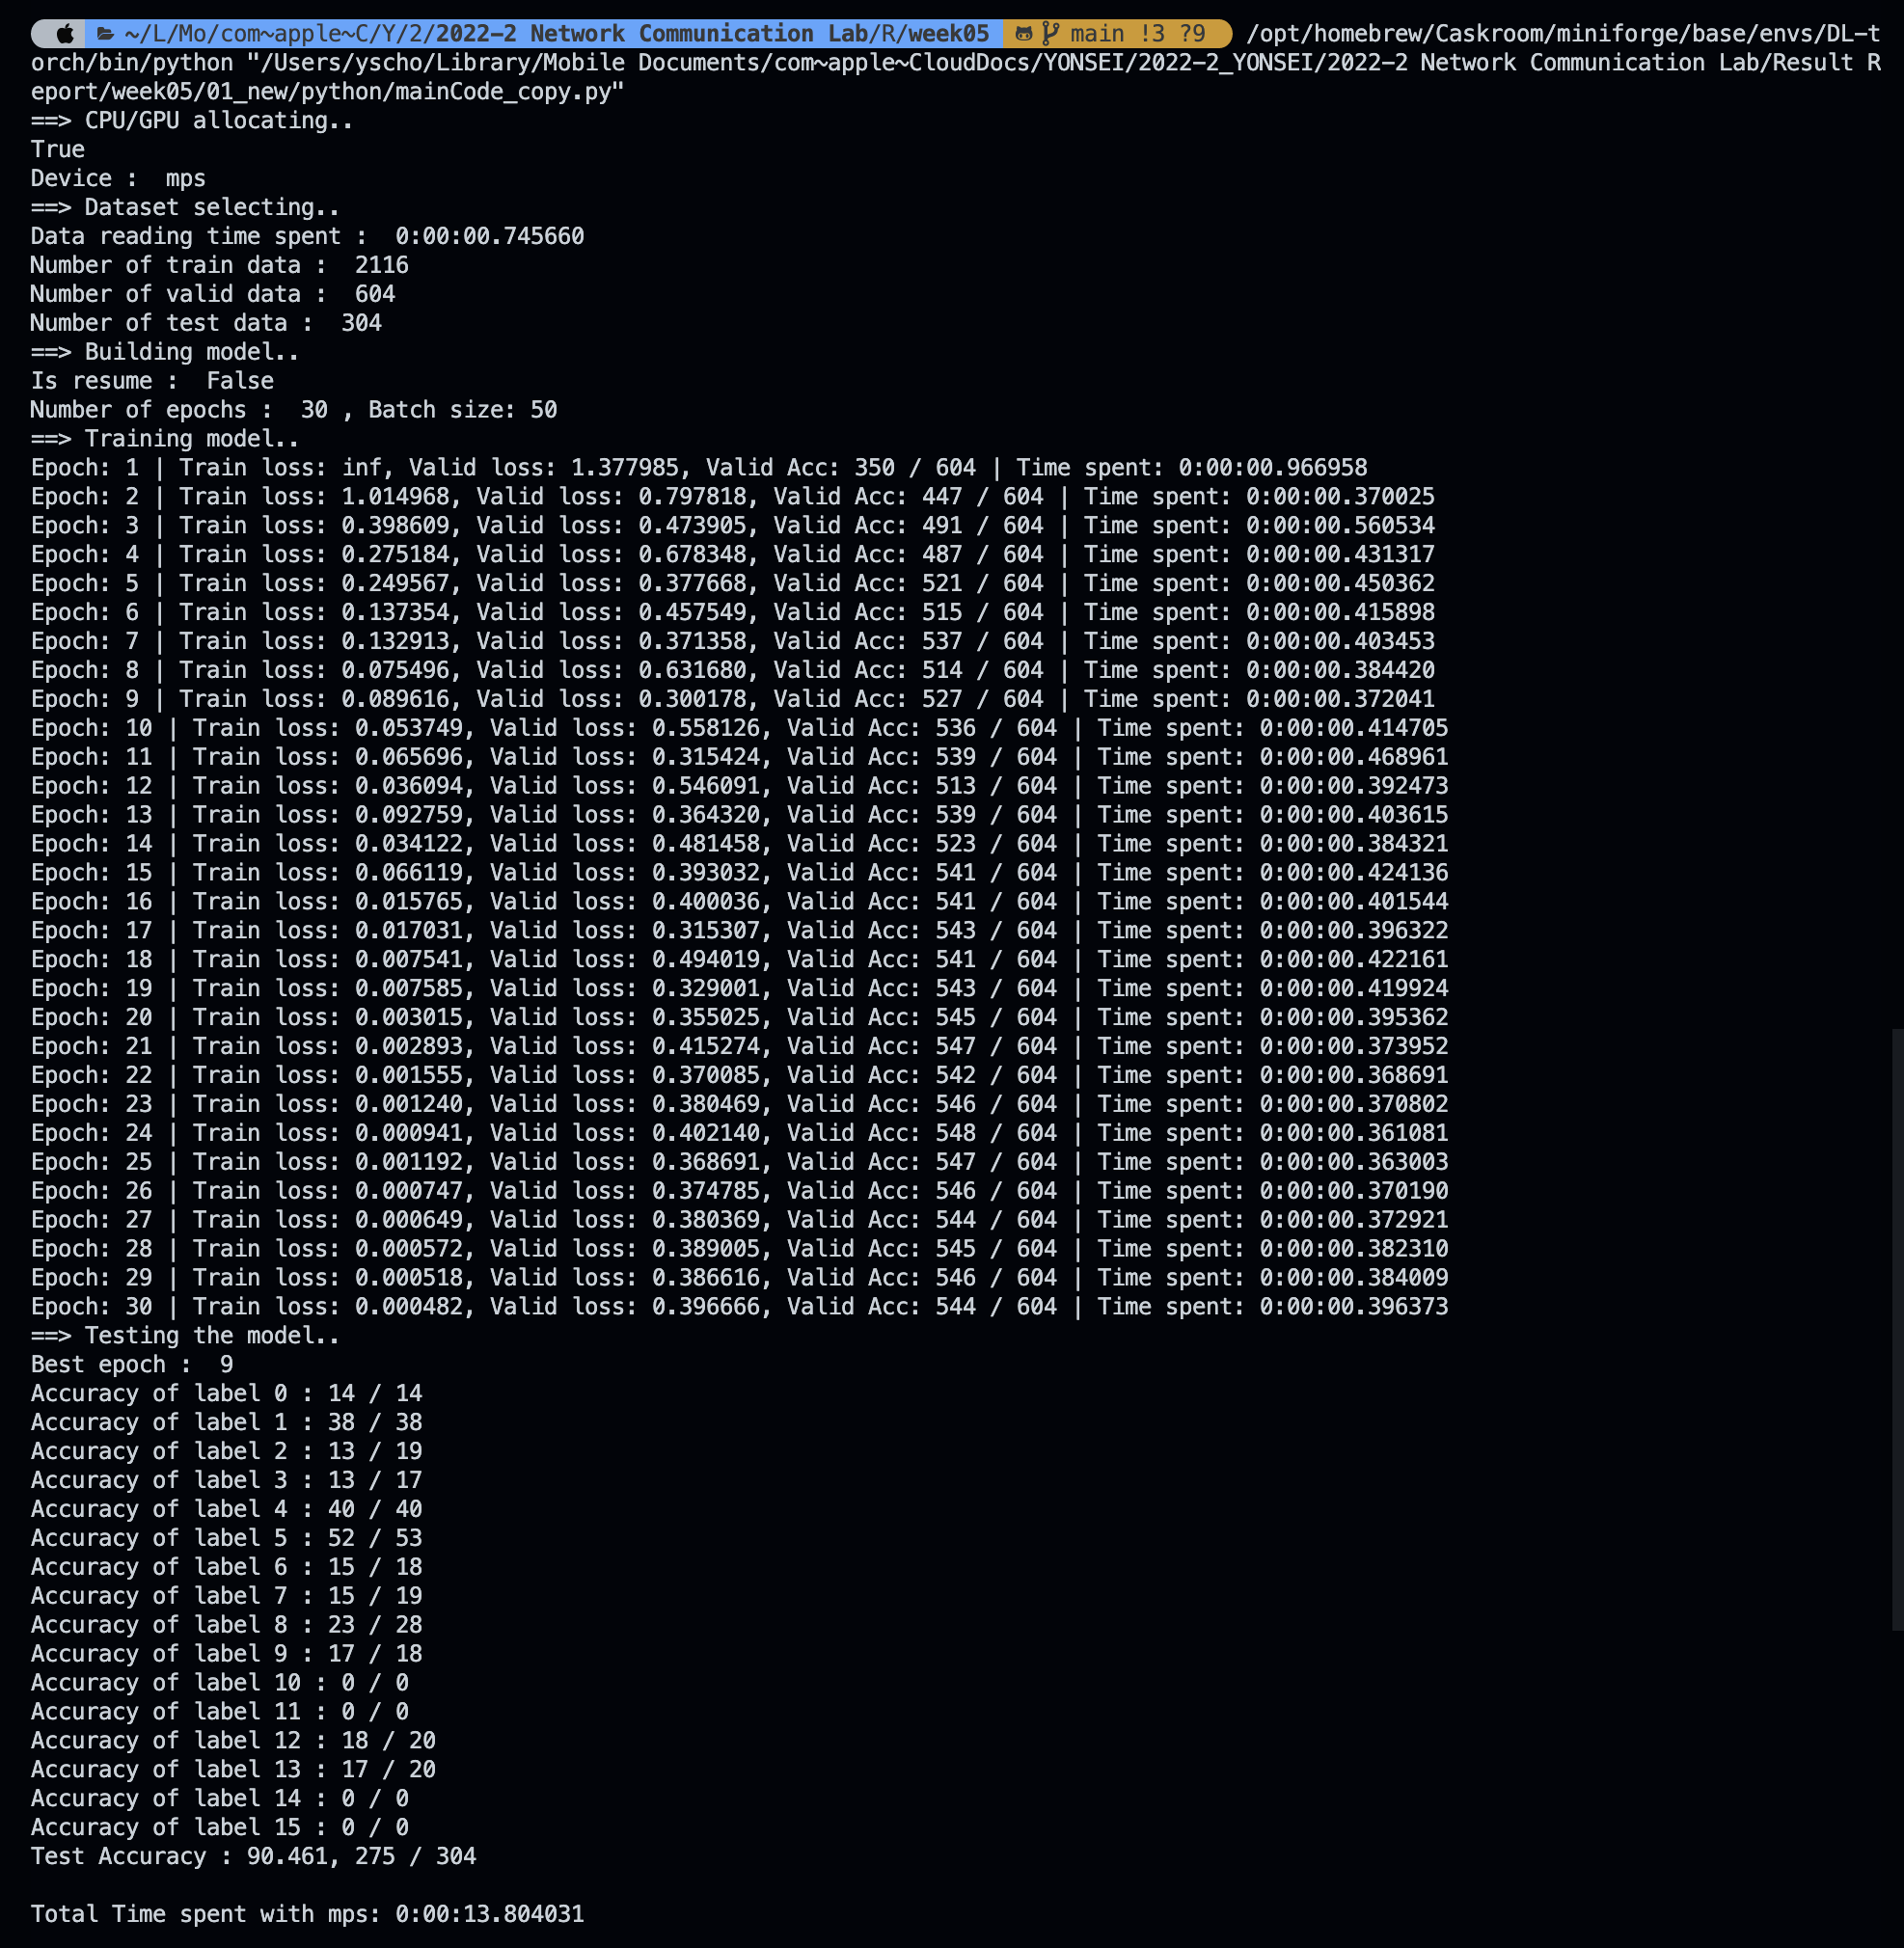
\includegraphics[width=.95\textwidth]{image/week05/2-1.png}
		\caption{\footnotesize 
		Terminal out results : Experiment 1, given dataset \& custom model}
		\vspace{-10pt}
    \end{figure}
\clearpage